\section{Praktyczna realizacja zadania}

\begin{figure}[h]
\centering
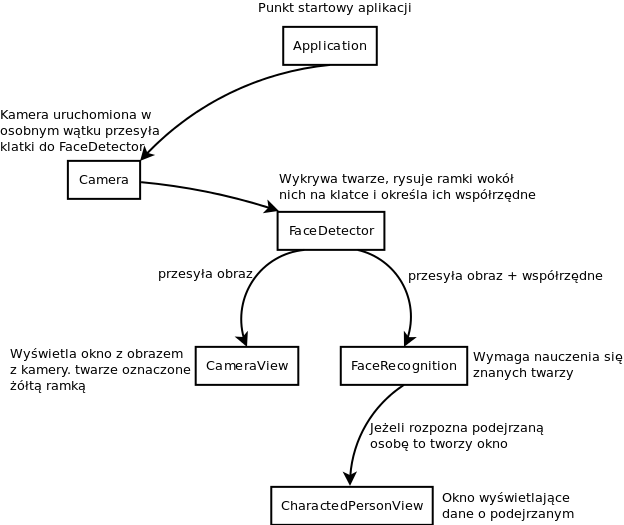
\includegraphics[scale=0.6]{./idea_dzialania_programu.png}
\caption[Idea działania programu]{Idea działania programu.}
\end{figure}

Obraz z kamery zostaje przekazany do klasy obserwatora, zostaje tam przetworzony, oraz następuje wychwycenie twarzy na zdjęciu. Interfejs graficzny otrzymuje przechwyconą klatkę z kamery, wraz z twarzami obramowanymi prostokątami i wyświetla obraz na ekranie. W tym samym czasie z klatki zostają wyodrębione wszystkie twarze, które są jednocześnie skalowane do rozmiaru 100\begin{math}\times\end{math}100 pikseli, a ich barwy są zmieniane do skali szarości. Dzięki wykorzystaniu wzorca projektowego obserwator, przy każdej zmianie obrazu na kamerze klasa otrzymuje nowy obraz, a natychmiast po przetworzeniu obrazu klasy nasłuchujące otrzymują wymagane dane (klatka z obramowaniem, wycięte twarze). 


\pagebreak[4]
